\section{Pruebas de Usabilidad}

Las pruebas de usabilidad se centran en evaluar la facilidad con la que los usuarios pueden interactuar con la aplicación. Para Argos, estas pruebas se realizaron sobre los mockups de alta fidelidad para obtener retroalimentación temprana y realizar ajustes antes de la fase de desarrollo, permitiendo iterar sobre el diseño de forma ágil y con un bajo costo.

\subsection{Plan de pruebas}

Se diseñó y ejecutó un plan de pruebas de usabilidad moderadas para observar directamente cómo los usuarios representativos interactúan con los prototipos de la aplicación al realizar una serie de tareas predefinidas.

\subsubsection{Alcance de pruebas}
El alcance de estas pruebas se limitó estrictamente a la \textbf{interfaz y experiencia de usuario (UI/UX)} de los mockups interactivos de la aplicación móvil de Argos. No se evaluó el rendimiento del backend, la seguridad de la base de datos ni la infraestructura de servidores. Las pruebas se enfocaron en los siguientes aspectos:
\begin{itemize}
	\item La eficiencia y tasa de éxito en la realización de los flujos de usuario principales (pase de lista, consulta de asistencia).
	\item La claridad y comprensión de la navegación, la arquitectura de la información y la terminología utilizada.
	\item La facilidad para localizar y utilizar funciones clave dentro de cada panel de usuario.
	\item La satisfacción subjetiva del usuario al interactuar con el prototipo.
\end{itemize}

\subsubsection{Objetivos de Pruebas}
Los objetivos cuantitativos y cualitativos de las pruebas fueron los siguientes:
\begin{itemize}
	\item \textbf{Validar el flujo de pase de lista:} Medir si un docente puede registrar la asistencia de una clase de 20 alumnos en menos de 3 minutos.
	\item \textbf{Evaluar la consulta de información:} Determinar si un estudiante y un padre de familia pueden encontrar y entender el reporte de asistencia detallado en menos de 1 minuto.
	\item \textbf{Identificar puntos de fricción:} Descubrir qué elementos de la interfaz, botones o secciones generan confusión, dudas o errores en la interacción.
	\item \textbf{Recopilar retroalimentación cualitativa:} Obtener opiniones, comentarios y sugerencias directas de los usuarios para mejorar la experiencia general de la aplicación.
\end{itemize}

\clearpage
\subsubsection{Entorno de pruebas}
Las pruebas se llevaron a cabo en un entorno controlado y neutral (un aula vacía en la UPP) para minimizar distracciones y simular un contexto de uso realista. Cada sesión individual contó con:
\begin{itemize}
	\item \textbf{Un participante:} Un usuario final real (estudiante, docente o padre de familia).
	\item \textbf{Un dispositivo móvil:} Un smartphone con el prototipo interactivo de los mockups cargado.
	\item \textbf{Un moderador:} Encargado de guiar la sesión, asignar las tareas y realizar preguntas.
	\item \textbf{Un observador:} Responsable de tomar notas detalladas sobre el comportamiento, las acciones y los comentarios del usuario.
\end{itemize}

\subsubsection{Resultados y/o Hallazgos}

Tras la ejecución de las pruebas con 5 participantes por cada rol, se consolidaron los siguientes hallazgos:

\begin{itemize}
    \item \textbf{Hallazgo 1 (Positivo):} El 85\% de los docentes participantes completaron la tarea de pase de lista dentro del tiempo objetivo, calificando el flujo como ``muy intuitivo y rápido''.
    \item \textbf{Hallazgo 2 (Mejora):} El 30\% de los estudiantes tardaron más de lo esperado en encontrar la opción para descargar su historial, sugiriendo que el botón podría tener una ubicación más prominente o un texto más claro.
    \item \textbf{Hallazgo 3 (Sugerencia):} El 60\% de los padres de familia sugirieron que la gráfica de asistencia en su panel debería permitir un filtro por semana, además del filtro mensual, para un seguimiento más granular.
    \item \textbf{Hallazgo 4 (Positivo):} El 85\% de los participantes comprendieron y utilizaron correctamente la navegación principal a través de la barra de pestañas inferior sin necesidad de guía, validando la arquitectura de la información.
\end{itemize}

\subsubsection*{Encuesta de Usabilidad y Experiencia de Usuario}

Con el objetivo de evaluar la usabilidad, accesibilidad y efectividad de las principales funciones de la plataforma, se aplicó una encuesta a tres grupos de usuarios: docentes, estudiantes y padres de familia.  

La encuesta se centró en identificar:
\begin{itemize}
    \item El nivel de facilidad para completar tareas clave (pase de lista, descarga de historial académico y navegación general).
    \item El grado de satisfacción con la experiencia de uso.
    \item Las principales sugerencias de mejora para optimizar la interacción con la plataforma.
\end{itemize}

Los resultados obtenidos permiten identificar fortalezas en la arquitectura de la información y áreas de oportunidad en la visibilidad de ciertas funciones, así como nuevas necesidades expresadas por los usuarios.



% Docentes y Estudiantes (fila 1)
\begin{figure}[H]
    \centering
    \begin{minipage}[b]{0.50\textwidth}
        \centering
        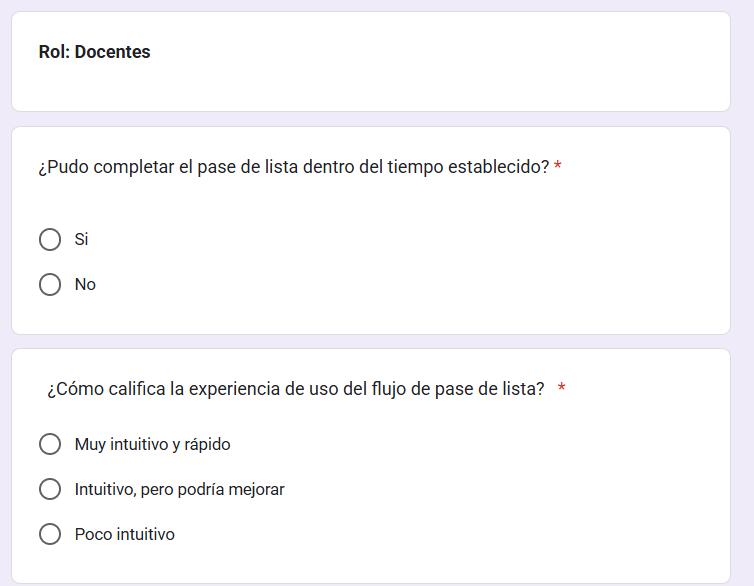
\includegraphics[width=1.0\textwidth]{./Media/p1.png}
        \caption{Encuesta aplicada a docentes.}
    \end{minipage}

    \begin{minipage}[b]{0.50\textwidth}
        \centering
        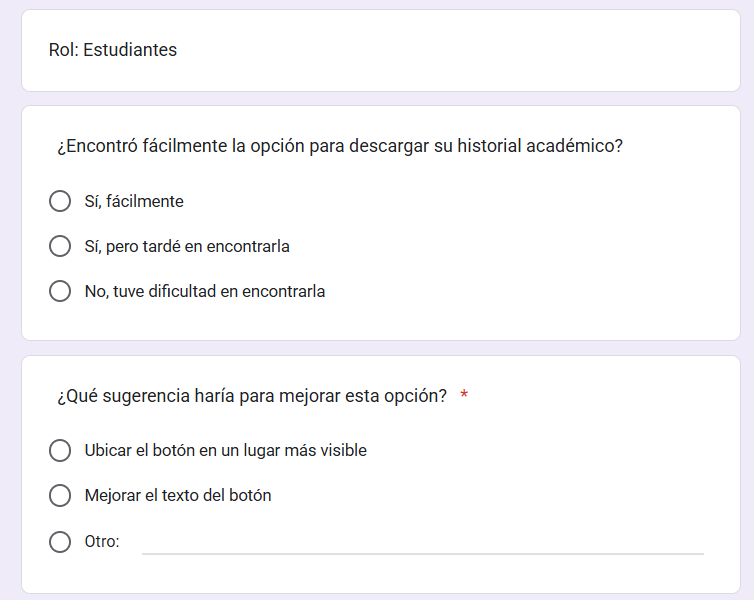
\includegraphics[width=1.0\textwidth]{./Media/p2.png}
        \caption{Encuesta aplicada a estudiantes.}
    \end{minipage}

     \centering
    \begin{minipage}[b]{0.50\textwidth}
        \centering
        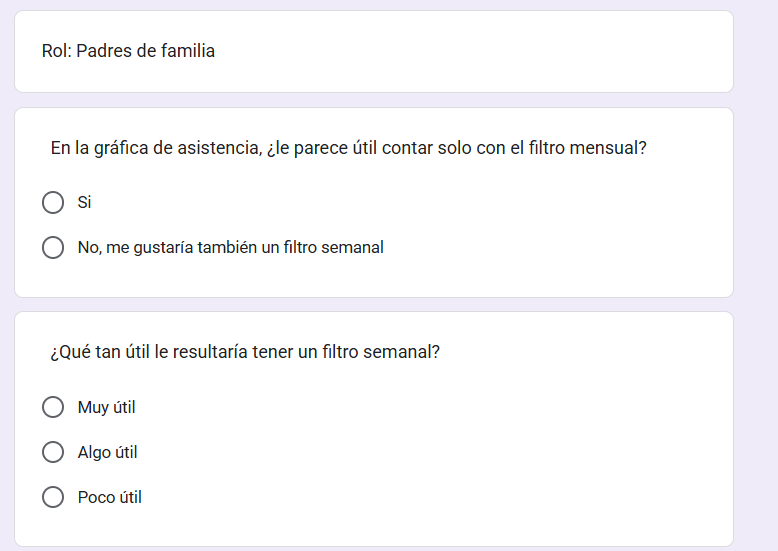
\includegraphics[width=1.0\textwidth]{./Media/p3.png}
        \caption{Encuesta aplicada a padres de familia.}
    \end{minipage}

\end{figure}


% Circulo (fila 3)
\begin{figure}[H]
    \centering
    \begin{minipage}[b]{0.65\textwidth}
        \centering
        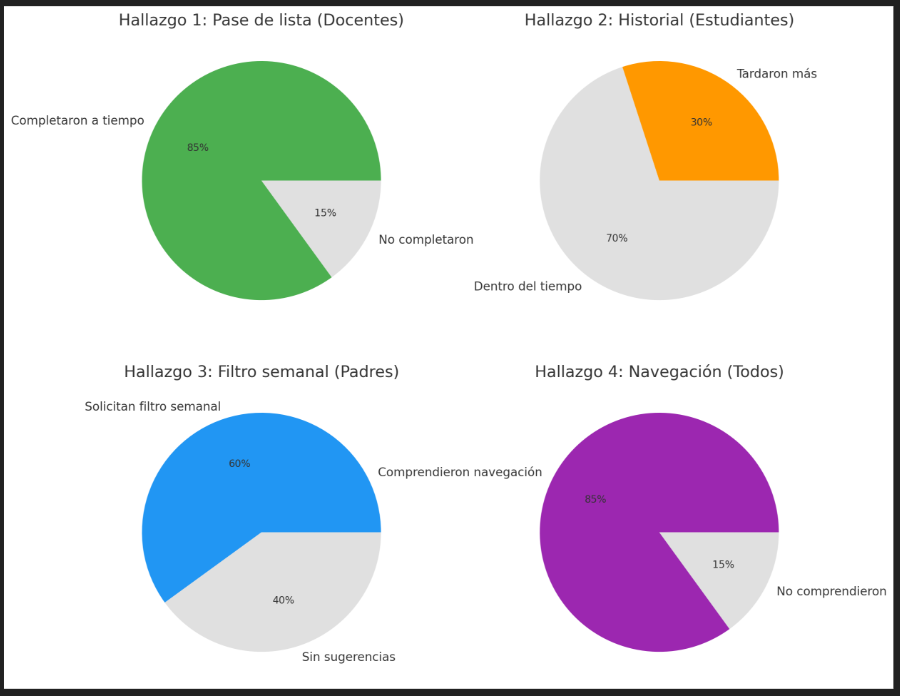
\includegraphics[width=1.0\textwidth]{./Media/Circulo.png}
        \caption{Gráfica comparativa circular de los hallazgos obtenidos en la encuesta.}
    \end{minipage}

     \centering
    \begin{minipage}[b]{0.65\textwidth}
        \centering
        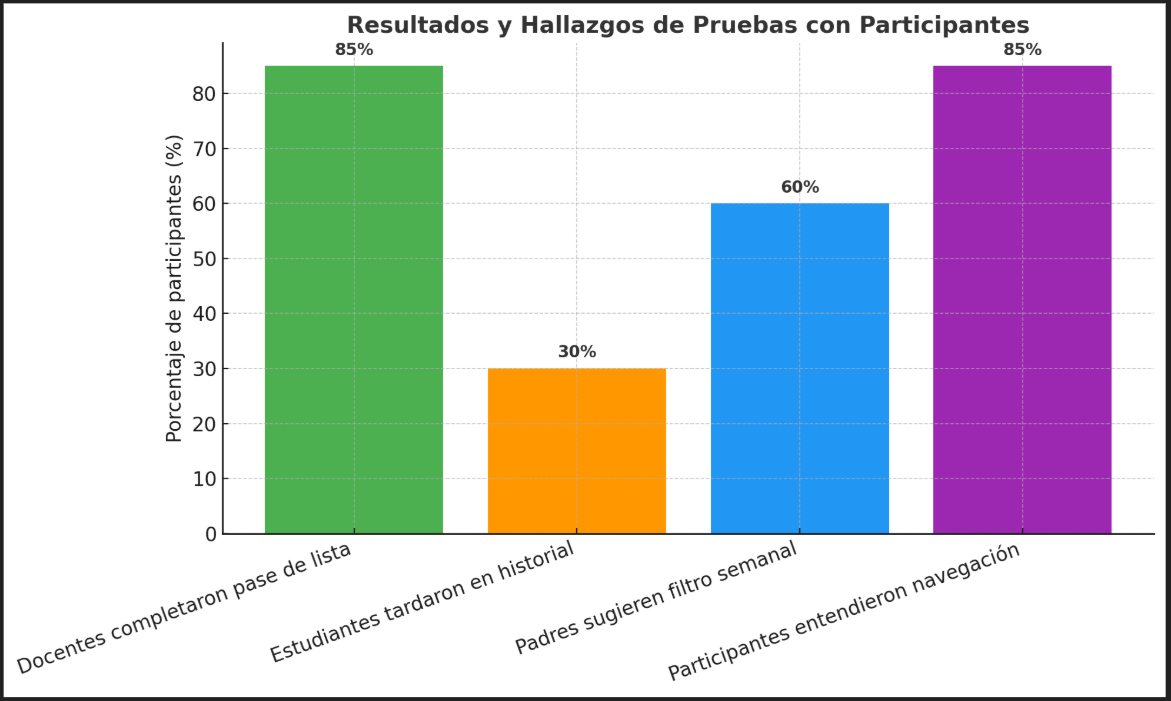
\includegraphics[width=1.0\textwidth]{./Media/Barras.png}
        \caption{Gráfica comparativa de barras de los hallazgos obtenidos en la encuesta.}
    \end{minipage}
\end{figure}


\subsubsection{Conclusión Final}
Las pruebas de usabilidad concluyeron que los flujos de trabajo principales de la aplicación Argos son sólidos, eficientes y fáciles de seguir para todos los roles de usuario. Los hallazgos permitieron identificar oportunidades de mejora específicas y de alto valor, principalmente en la visibilidad de funciones secundarias y en la flexibilidad de los filtros de datos. Las recomendaciones, como rediseñar la ubicación del botón de descarga y añadir un filtro semanal en el panel de padres, serán incorporadas en la siguiente iteración del diseño antes de proceder con el desarrollo.